\begin{figure*}
  \centering
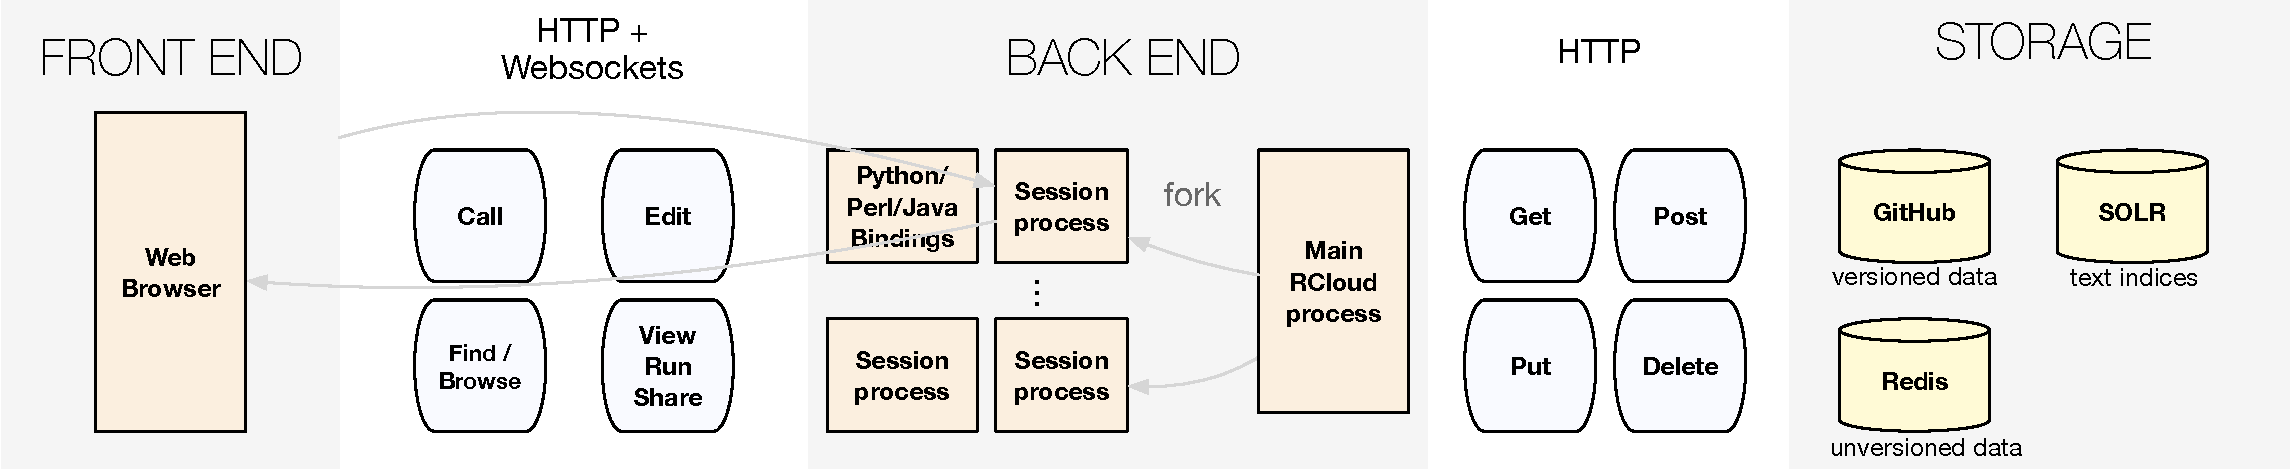
\includegraphics[width=.75\linewidth]{fig/system/system.pdf}
\caption{\label{fig:system}A diagram of RCloud's architecture. }
\end{figure*}

\section{Related Work}

\stephen{In addition to the immense foundation of work on systems
for statistical computing,}
There is much previous work that inspired or influenced ours.
Indeed, many studies have addressed requirements for future visual
analytics environments.
Previous work that we learned from includes:

{\bf VisTrails} as a landmark prototype of a scientific workflow
and provenance management system. This prototype demonstrated
the value of capturing aspects of the processes that
surround data analysis experiments and tools, including detailed
history, collaboration, and deployment.

{\bf iPython notebooks (Jupyter)} are the closest work we are aware of.
The goal of this project is to provide shared notebooks and a remote
execution environment for interpreted scripts. 
\stephen{Are there significant differences involving versioning,
provenance, annotation and other broad process support?}

{\bf RStudio, RShiny} and other packages based on R for creating and
publishing web content such as knitR, Rpubs, rCharts, and gg2v.
These tools are not collaborative, but they are aimed at better
graphics and web applications.

{\bf bl.ocks, jsfiddle, plotly} and other web services for sharing code
and demos.

Further afield, {\bf Electronic Lab Notebooks} are applications for organizing
and sharing data from scientific lab experiments\cite{Rubacha:2011:ELN}.
In a sense, we hope to adapt and extend this concept to the work of
visual analytics teams.

Kandel et al.'s interview study points out the typical ``explore'',
``model'', ``report'' cycle in enterprise data
analysis~\cite{Kandel:2012:EDA}. There are many discontinuities in
this cycle that cost time and effort to overcome. RCloud seeks to
reduce this mismatch. Kandel et al also point out that larger teams
are becoming more common in data analysis, that supporting
collaboration is difficult and important, and that sharing
and versioning of data sources and artifacts is hindered by current
technology. ``We found that analysts typically did not
share scripts with each other. Scripts that were shared were
disseminated similarly to intermediate data: either through shared
drives or email. Analysts rarely stored their analytic code in source
control.'' Their study highlights the opportunity for better ways
of supporting collaboration and sharing in data analysis teams.

An earlier study by Kandel et al argues that data wrangling
(cleaning, parsing and transformation)is a major part of exploratory
analysis and visualization~\cite{Kandel:2011:RDI}. We view this
as attacking a different semantic level than ours, but also
showing the need for an environment that enables better sharing
of the knowledge, tools and processes to do this. Anecdotally
we find much frustration among practitioners that this knowledge
is difficult to find and often isnot recorded or available in a
reusable form even within the same organization.

Heer and Agarwala identify many design considerations for
collaborative visual analytics~\cite{Heer:2008:DCF}.
RCloud notebooks, and the integrated version control system for them,
described in Section~\ref{sec:notebooks}, address modularity and granularity,
and artifact histories.
\emph{Starring}, the means for signaling interest in notebooks, described in
Section~\ref{sec:starring}, addresses social-psychological incentives,
recommendation, and voting and ranking. RCloud's integrated deployment
mechanism, described in Section~\ref{sec:deployment}, addresses the cost of
integration, content export, presentation and view sharing.

{\bf Manyeyes} \cite{Viegas:2007:MAS} was a landmark system for the integration
of social media with visualization and data publishing. We build on this
work by defining a rich interface for collaboration about code, and for
operating on metadata.

The need for integrating statistics and visualization has been
highlighted in previous studies and is widely understood by
various technical communities \cite{Perer:2008:ISA}
Lucas and Roth were early advocates of combining
data exploration with presentation and publication \cite{Lucas:1996:EIV}.

There has been noteworthy work on specific techniques such as
social bookmarking \cite{Millen:2006:DSB} \cite{Heer:2007:VAV}
and crowdsourcing \cite{Fast:2014:ECS} to support collaborative
or social development or analysis processes.
Similarly, there are computational methods to support high
performance execution in incremental code development
environments \cite{Guo:2010:TPI}.
The goal of RCloud is to define an environment in which many such
techniques may be integrated and made available to a broad community.

{\bf VisMashup}~\cite{Santos:2009:VST} and Crowdlabs~\cite{Mates:2011:CSA}
are tools built on top of the VisTrails workflow management
system~\cite{Callahan:2006:VVM}. VisMashup defines a schema and
semantics for automatically deriving user interfaces from workflows,
while Crowdlabs exposes these capabilities on a website feature
workflow upload and remote execution. In our view, the impedance
mismatch between a dataflow pipeline specification and the power of a
general-purpose language is too great for the type of general
exploratory work in data science teams. As a result, RCloud tries to
provide a closer match for analysts accustomed to creating and
executing R and Python code, while retaining attractive
properties like automatic versioning and management.

\begin{figure*}
\centering
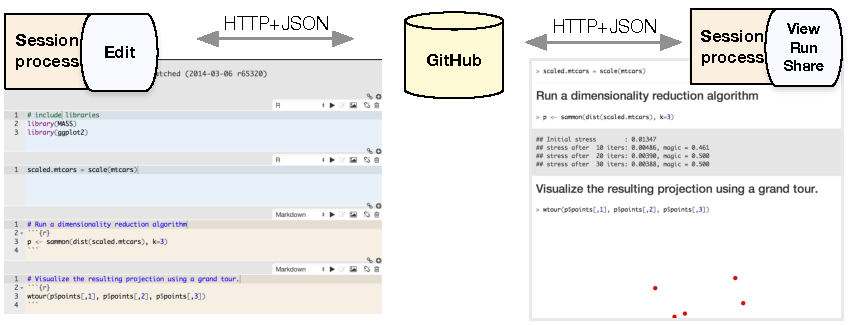
\includegraphics[width=.8\linewidth]{fig/notebook/notebook.pdf}
\caption{\label{fig:notebook}An RCloud notebook is a sequence of
  \emph{cells}, each a snippet of source in R or Markdown. Notebooks
  are stored in GitHub \emph{gists}, which provide the version-control
  primitives needed in RCloud during editing (left) or viewing and
  executing (right).}
\end{figure*}

Our work has been inspired by and benefited from other efforts
to improve data analysis environments and processes,
including RStudio \cite{RStudio:2013:SWA},
the R packages Markdown \cite{Allaire:2014:MMR},
knitr \cite{Xie:2013:DDW}
and Shiny \cite{RStudio:2013:SWA},
and iPython notebooks \cite{Perez:2007:IAS}
to name a few. RStudio aims at providing an integrated development environment
for R, with support for publishing code in packages. Markdown,
knitR and Shiny augment R with sophisticated reporting capabilities, including
interactive web interfaces. IPython \cite{Perez:2007:IAS}
shares many of our goals, such as providing a comprehensive environment
for analysis and programming, and share-able documents on the web.
\stephen{Do we now need to introduce one of those remarks where we
explain that we are not the same as IPython.}

One overall goal is to reduce the gap between implementers and deployers
of technology in visual analytics. The fusion of development with production
operations in software release management (``DevOps'' \cite{Httermann:2012:DD}
or ``continuous integration'' \cite{Fowler:2006:Continuous}) is a trend in web
services and related fields.
By making it convenient for data scientists to expend just a little more effort
in the process of creating experiments, we may be able to eliminate the need
for programming teams to recreate their work in production, which has a high
penalty in time, expense and accuracy.
